\chapter{Ten micrometres: designing the run}\label{ch:ten}

Everything so far went from 3\um\ to 0.5\um. A real QDM often sits further from the sample. The last question of the
project was: can the 0.5\um\ field be reconstructed from a measurement at \textbf{10\um}? This chapter is about the
design, and the next about the results. The full record with every table is \code{README_HIGH_STANDOFF.md}, in the phase 9 folder of
\code{final_evaluation/02_source_docs}.

\section{Why 10\um\ is a different problem}

The blur is $e^{-k\,\Delta z}$, and now $\Delta z=9.5$\um\ instead of 2.5.

\begin{center}
\begin{tabular}{lcc}
\toprule
A pattern that repeats every & keeps, over 2.5\um & keeps, over 9.5\um \\
\midrule
40\um & 68\% & 22\% \\
10\um & 21\% & 0.3\% \\
4\um & 2\% & $3\times10^{-7}$ \\
\bottomrule
\end{tabular}
\end{center}

\begin{figure}[H]
\centering
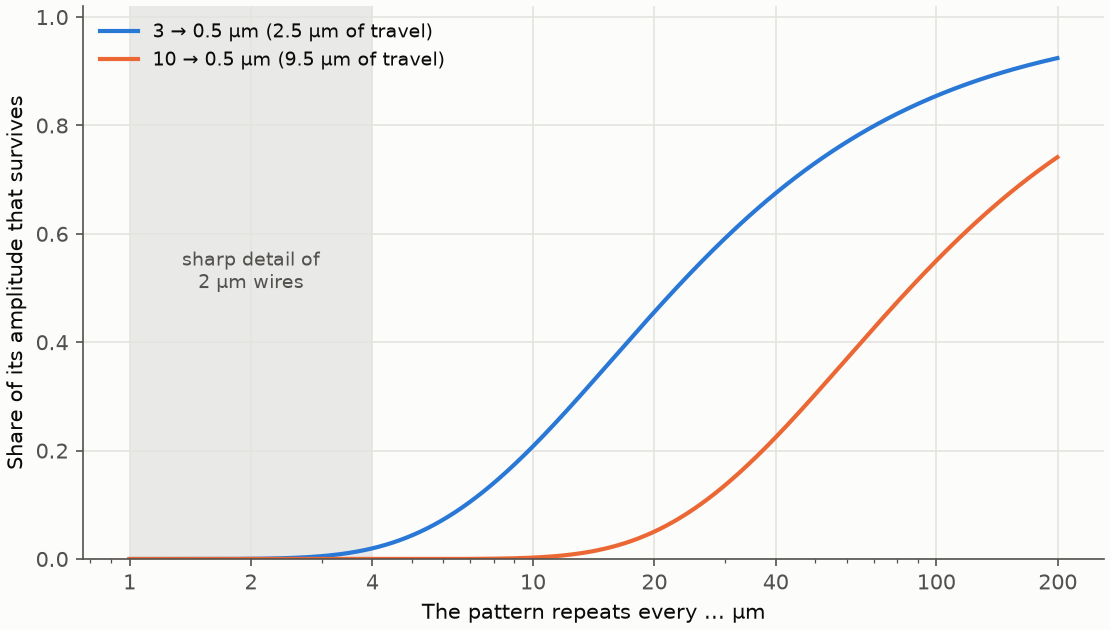
\includegraphics[width=0.75\textwidth]{late_decay}
\caption{How much of each pattern survives the blur, for the two problems. Wires 2\um\ wide have most of their sharp detail
far to the right of what survives at 10\um.}
\label{fig:late_decay}
\end{figure}

At 3\um\ a wire edge is weakened. At 10\um\ it is gone. On the COMSOL coils, 56\% (\code{L1_C1}) and 73.5\%
(\code{IC_4um}) of the 0.5\um\ field's norm lies where the 10\um\ measurement carries nothing (Chapter~\ref{ch:floor}). In
the language of Chapter~\ref{ch:limits}: the measured band has shrunk to almost nothing and nearly everything is prior
band. A method that only inverts the blur is stuck near 56--73\%. Only knowledge of what sources look like can do
better.

The existing networks do not reach. On simulated images at 10\um, run 2 scores 92\% and run 3 scores 56.8\%.

\section{How MAGIC-UNet sees a large image}

To understand the design you first need a piece of code that this booklet has not shown yet. The network only accepts
$64\times64$ images. A full image is $1400\times1400$. So it is cut into overlapping tiles, each tile is processed
alone, and the results are stitched.

Where the tiles start:

\begin{code*}{magic_unet.py}
def tile_starts(size, tile, stride):
    starts = list(range(0, size - tile + 1, stride))
    if starts[-1] != size - tile:
        starts.append(size - tile)
    return starts
\end{code*}

With a stride smaller than the tile, neighbours overlap. In the overlap, two tiles have each made a prediction. Which
one is kept? Each pixel goes to the tile whose \emph{centre} is nearest, because a network is most reliable in the middle
of its view and least at the edges:

\begin{code*}{magic_unet.py}
    pos = np.arange(size)[:, None]
    s = np.asarray(starts)[None, :]
    covers = (pos >= s) & (pos < s + tile)
    dist = np.where(covers, np.abs(pos - (s + (tile - 1) / 2)), np.inf)
    return np.asarray(starts)[dist.argmin(1)]
\end{code*}

And each tile is scaled by its own largest field before it enters the network, and scaled back afterwards:

\begin{code*}{magic_unet.py}
        x = torch.stack([full[:, r:r + tile, c:c + tile] for r, c in part])
        a = alpha(x).clamp_min(1e-30)
        y = model((x / a[:, None, None, None]).to(device)).cpu().double()
        y = y * a.double()[:, None, None, None] / beta
\end{code*}

\begin{keyidea}[The one fact that matters for 10\um]
Each tile is processed \textbf{alone}. The network sees 64 pixels by 64 pixels of field and nothing else. Whatever lies
outside that window does not exist for it.
\end{keyidea}

\section{The tile is too small at 10\um}

With 0.2\um\ pixels a tile is 12.8\um\ wide. At 3\um\ that is about four standoffs. At 10\um\ it is \emph{narrower than the
blur itself}, which is 15--20\um\ wide. The field inside such a tile is made mostly by wires that are not in it.

This can be measured with no network at all. Take a simulated layout. Keep only the current inside one tile and compute
its field. Compare with the field of the whole layout, inside the same tile. The difference is the part that comes from
outside:

\begin{code*}{tile_context_check.py}
            mx, my = np.zeros_like(jx), np.zeros_like(jy)
            mx[r:r + n, c:c + n], my[r:r + n, c:c + n] = jx[r:r + n, c:c + n], jy[r:r + n, c:c + n]
            inside = biot_savart_sheet(mx, my, dx, z)
            num = sum(np.sum((full[z][k][r:r + n, c:c + n] - inside[k][r:r + n, c:c + n]) ** 2) for k in range(3))
            den = sum(np.sum(full[z][k][r:r + n, c:c + n] ** 2) for k in range(3))
            out[(z, w)].append(np.sqrt(num / den))
\end{code*}

\code{mx, my} is the current with everything outside the tile set to zero. \code{full} is the field of the whole layout.
The last line is the share of the tile's field that the tile's own current cannot explain.

\begin{center}
\begin{tabular}{llc}
\toprule
Standoff & Tile & Share of the tile's field from currents outside it \\
\midrule
3\um\ (run 2) & 12.8\um & 50\% \\
8\um & 12.8\um & 70\% \\
10\um & 12.8\um & \textbf{78\%} \\
10\um & 25.6\um & 60\% \\
10\um & 44.8\um & \textbf{52\%} \\
\bottomrule
\end{tabular}
\end{center}

Each number is the median over 12 tiles from 4 layouts, and single tiles vary widely (for example 48--123\% at 10\um\ with
the small tile), so read the trend, not the digits. At 10\um\ with the old tile, four fifths of what the network sees was made by something it cannot see. A 44.8\um\ tile
brings the share back to run 2's.

\begin{figure}[H]
\centering
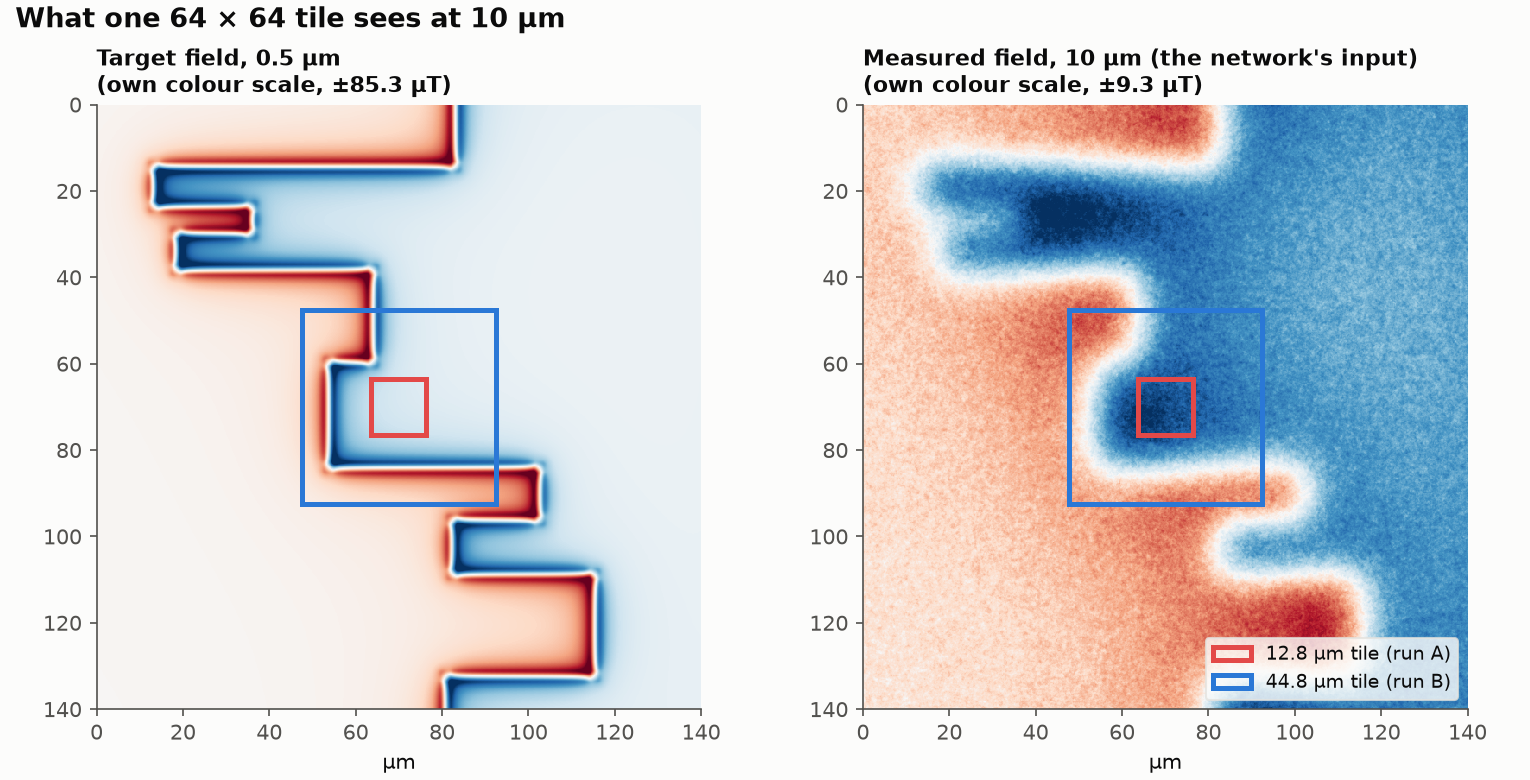
\includegraphics[width=0.92\textwidth]{hs_tile_context}
\caption{The target at 0.5\um\ and the measured field at 10\um\ for one test layout, with both tile sizes drawn on them.
Inside the small tile the measured field is almost featureless.}
\label{fig:hs_tiles}
\end{figure}

\section{Bigger pixels, not a bigger network}

How do you make a 44.8\um\ tile without changing the network? The network must stay $64\times64$: you asked for the
paper's architecture, unmodified. So keep 64 pixels and make each pixel larger: $44.8/64=0.7$\um. The simulator works
at 0.1\um, so 7 by 7 of its pixels are averaged into one:

\begin{code*}{magic_data.py}
def binned(a, factor):
    """Area average over factor x factor pixels; a: [..., H, W]."""
    if factor == 1:
        return a
    *lead, h, w = a.shape
    return a.reshape(*lead, h // factor, factor, w // factor, factor).mean((-3, -1))
\end{code*}

Run 2 already did this with \code{factor = 2}. Averaging pixels is what a camera does when it bins.

At inference the same averaging is applied to the measured field, the network predicts a current on the coarse grid,
and the current is copied back onto the fine grid before the physics step:

\begin{code*}{train_magic_unet.py}
    j = predict_tiled(model, binned(np.asarray(b, np.float64), factor), beta, args.tile, stride,
                      args.infer_batch, device)
    j = np.kron(j, np.ones((1, factor, factor)))
    return field_from_sheet(j, height, DX), j
\end{code*}

\code{np.kron} with a block of ones repeats each coarse pixel $7\times7$ times. The score is then taken on the full
$1400\times1400$ image at 0.1\um, exactly as for every other method.

\begin{careful}[What bigger pixels cost]
A current drawn on 0.7\um\ pixels cannot have edges sharper than 0.7\um. Measured with a \emph{perfect} current and no
network: 2.2\% error with 0.2\um\ pixels, 3.1\% with 0.5\um, 4.6\% with 0.7\um. So run B starts 2.4 points behind before
it has learned anything. The bet was that seeing the wires is worth far more than that.
\end{careful}

\section{The standoff band}

Run 3 broke at 10\um\ because 10\um\ was the \emph{edge} of its range (Chapter~\ref{ch:run3}). So the new runs put 10\um\ in
the middle: a normal distribution around 10\um\ with a spread of 2\um, cut at three spreads, which gives 4 to 16\um. It is
the same 20\% spread as run 2's $3\pm0.6$\um\ (and as our reading of the paper's $50\pm10$\um), and it uses the code path of
Chapter~\ref{ch:run3} with \code{--z-mean 10 --z-std 2}. As always, the network is never given the value.

\section{Two runs that differ in one thing}

\begin{center}
\begin{tabular}{lcc}
\toprule
 & Run A (control) & Run B \\
\midrule
Training standoff & \multicolumn{2}{c}{$10\pm2$\um, never given to the network} \\
Pixels & 0.2\um\ (\code{--bin 2}) & 0.7\um\ (\code{--bin 7}) \\
Tile & 12.8\um & 44.8\um \\
Training crops & \multicolumn{2}{c}{4{,}800 layouts $\times$ 4 standoffs $\times$ 8 crops $=$ 153{,}600} \\
Network and recipe & \multicolumn{2}{c}{unmodified, the paper's: RMSprop, $10^{-4}$, 50 epochs, batch 32} \\
\bottomrule
\end{tabular}
\end{center}

Run A is run 2 with only the standoff changed. Run B is run A with only the pixel size changed. If B beats A, the
pixel size is the reason, and nothing else can be.

\begin{careful}[What is ours here]
The network and the training recipe are the paper's. The two pixel sizes and the split into 4{,}800 layouts with 8 crops
per standoff are our choices. Run 2 used 2{,}400 layouts with 16 crops per standoff; the total number of crops is the
same, 153{,}600.

The pixel-size change was made for MAGIC-UNet only. When CSC-LISTA and FISTA-Net were later run at 10\um, they kept
their 3\um\ settings, so the 10\um\ method comparison is not like-for-like (Section~\ref{sec:fair}).
\end{careful}

\section{The rules, written first}

As in Chapter~\ref{ch:fista_depth}, the rules were fixed and hashed before either run was launched. They are in
the file \code{HIGH_STANDOFF_PROTOCOL.md}:
\begin{itemize}
\item \textbf{Main test:} 50 held-out \emph{simulated} layouts at 10\um, scored at full resolution. The same layouts at 6, 8,
12 and 14\um\ show the range.
\item \textbf{Second test:} the 15 COMSOL pairs at 10\um. Nothing is chosen on them, and they are reported with the warning
of Chapter~\ref{ch:comsol}.
\item \textbf{A against B:} the lower simulated error wins; under one point is a tie.
\item \textbf{Baseline:} FISTA, with everything about it chosen on simulation.
\end{itemize}

\begin{keyidea}[Why the main test is simulation this time]
At 3\um\ COMSOL was a fair test and we kept it as the judge. At 10\um\ Chapter~\ref{ch:comsol} showed that COMSOL's field
is not the field a real coil would make. Judging a physically trained network by it would be judging it against an
artefact. So the judge is free-space simulation, on layouts the network has never seen, and COMSOL is shown beside it.
The re-solve of 17 November (Chapter~\ref{ch:comsol}) confirmed the choice: the 10\um\ COMSOL inputs that were scored
are 39--58\% away from a correctly solved field, while the free-space simulator matches the re-solve to 3--9\%.
\end{keyidea}

Six amendments followed, each dated and written before the number it affects: details of the FISTA baseline (A1 to A3),
a server crash and restart (A4), a check added afterwards (A5), and the other learned methods at 10\um\ (A6).

\section{A crash, and a bug that had never been run}

On 15 November the server ran out of memory and was rebooted. Run A had finished. Run B was killed during its last
epoch, with 49 of 50 saved. The trainer saves a checkpoint after every epoch and can continue from it:

\begin{code*}{train_magic_unet.py}
        state = torch.load(latest, map_location=device, weights_only=False)
        model.load_state_dict(state['model'])
        optimizer.load_state_dict(state['optimizer'])
\end{code*}

The first attempt to resume stopped at once. The checkpoint also stores the state of the random number generator, and
\code{map_location=device} had moved \emph{everything} in the file to the GPU, including that state, which PyTorch only
accepts on the CPU. One word fixed it:

\begin{code*}{train_magic_unet.py}
        torch.set_rng_state(state['torch_rng'].cpu())      # map_location moved it to the GPU
\end{code*}

\begin{careful}[The lesson]
The restart path had existed since run 2 and had never once been used on the GPU. Code that has never run is code
that does not work yet. The fix does not touch training or scoring, and it is recorded in amendment A4. One honest
detail: after the restart the last epoch drew different training noise than an uninterrupted run would have.
\end{careful}

\begin{defend}[If your professor asks: did you change the network for 10\um?]
No. It is the same 15{,}505{,}194 parameters and the same training recipe. What changed is the data: the standoff
band, and the pixel size, so that 64 pixels cover 44.8\um\ instead of 12.8\um. Both are labelled as our choices.
\end{defend}

\begin{defend}[If your professor asks: why 0.7\um\ pixels and not some other number?]
Because of a measurement made before training. At 10\um\ a 12.8\um\ tile gets 78\% of its field from wires outside it; a
44.8\um\ tile gets 52\%, the same as run 2 had at 3\um. 44.8\um\ over 64 pixels is 0.7\um. And we ran the 0.2\um\ version too,
as the control, so the claim rests on a comparison and not on the argument.
\end{defend}
